\documentclass[tikz,border=10pt]{standalone}
\begin{document}
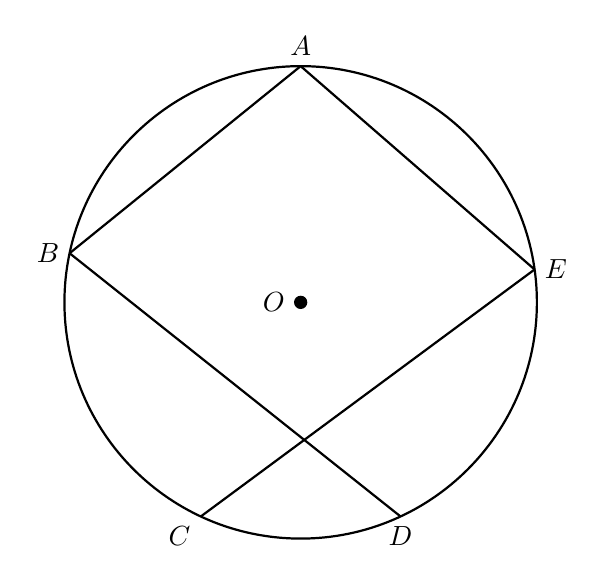
\begin{tikzpicture}[scale=2,thick]
  \coordinate (O) at (0,0);
  \coordinate (A) at (90:1.5);
  \coordinate (B) at (168:1.5);
  \coordinate (E) at (8:1.5);
  \coordinate (C) at (245:1.5);
  \coordinate (D) at (295:1.5);

  \draw (O) circle (1.5);
  \draw (A) -- (B);
  \draw (B) -- (D);
  \draw (A) -- (E);
  \draw (E) -- (C);

  \fill (O) circle (1.2pt);

  \node[above] at (A) {$A$};
  \node[left] at (B) {$B$};
  \node[right] at (E) {$E$};
  \node[below left] at (C) {$C$};
  \node[below] at (D) {$D$};
  \node[left=2pt] at (O) {$O$};
\end{tikzpicture}
\end{document}
